\documentclass{mp}
\usepackage[linesnumbered]{algorithm2e}
\DontPrintSemicolon
\graphicspath{{15_prng}}
\subtitle{Generatory liczb pseudolosowych\\(wykład skrócony)}

\SetKwProg{Fn}{Function}{}{end}
\SetKwInput{Assert}{assert}

\usepackage{alltt}

\usepackage{listings}
\lstdefinelanguage{C99}[]{C}{morekeywords={uint64\_t, uint32\_t, uint16\_t}}

\usepackage{tikzsymbols}

\newcommand{\xor}{\oplus}
\renewcommand{\vec}[1]{\mathbf{#1}}
\newcommand{\diag}[1]{\vec{D_{#1}}}

\makeatletter
\lst@Key{linebackgroundcolor}{}{}
\makeatother

%\usepackage{lstlinebgrd} % see http://www.ctan.org/pkg/lstaddons
%
%%http://tex.stackexchange.com/questions/8851/how-can-i-highlight-some-lines-from-source-code
%\makeatletter
%%%%%%%%%%%%%%%%%%%%%%%%%%%%%%%%%%%%%%%%%%%%%%%%%%%%%%%%%%%%%%%%%%%%%%%%%%%%%%%
%%
%% \btIfInRange{number}{range list}{TRUE}{FALSE}
%%
%% Test in int number <number> is element of a (comma separated) list of ranges
%% (such as: {1,3-5,7,10-12,14}) and processes <TRUE> or <FALSE> respectively
%
%\newcount\bt@rangea
%\newcount\bt@rangeb
%
%\newcommand\btIfInRange[2]{%
%    \global\let\bt@inrange\@secondoftwo%
%    \edef\bt@rangelist{#2}%
%    \foreach \range in \bt@rangelist {%
%        \afterassignment\bt@getrangeb%
%        \bt@rangea=0\range\relax%
%        \pgfmathtruncatemacro\result{ ( #1 >= \bt@rangea) && (#1 <= \bt@rangeb) }%
%        \ifnum\result=1\relax%
%            \breakforeach%
%            \global\let\bt@inrange\@firstoftwo%
%        \fi%
%    }%
%    \bt@inrange%
%}
%\newcommand\bt@getrangeb{%
%    \@ifnextchar\relax%
%        {\bt@rangeb=\bt@rangea}%
%        {\@getrangeb}%
%}
%\def\@getrangeb-#1\relax{%
%    \ifx\relax#1\relax%
%        \bt@rangeb=100000%   \maxdimen is too large for pgfmath
%    \else%
%        \bt@rangeb=#1\relax%
%    \fi%
%}
%
%%%%%%%%%%%%%%%%%%%%%%%%%%%%%%%%%%%%%%%%%%%%%%%%%%%%%%%%%%%%%%%%%%%%%%%%%%%%%%%
%%
%% \btLstHL<overlay spec>{range list}
%%
%% TODO BUG: \btLstHL commands can not yet be accumulated if more than one overlay spec match.
%% 
%\newcommand<>{\btLstHL}[1]{%
%  \only#2{\btIfInRange{\value{lstnumber}}{#1}{\color{color4!30}\def\lst@linebgrdcmd{\color@block}}{\def\lst@linebgrdcmd####1####2####3{}}}%
%}%
%\makeatother



\begin{document}
\frame{\titlepage}
\begin{frame}{Agenda}
\tableofcontents
\end{frame}

\section{Wprowadzenie}

\begin{frame}{9}
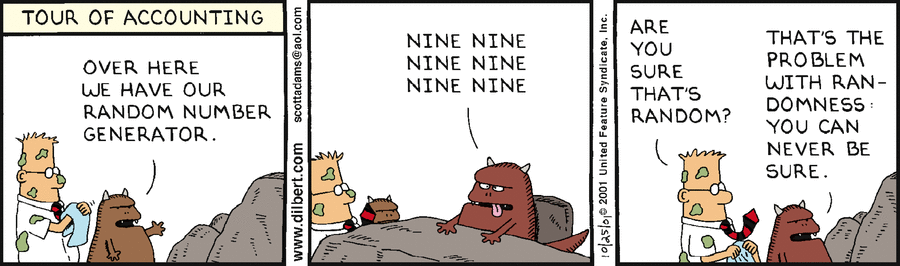
\includegraphics[width=\textwidth]{15_prng/dilbert.png}
\vfill
{\small \url{http://dilbert.com/strip/2001-10-25}}
\end{frame}
\begin{frame}{Ciąg liczb losowych}
\[ (X_1, X_2, \ldots) \]
\pause
\begin{enumerate}
\item $X_i$ mają identyczne rozkłady
\item $X_i$ są niezależne
\end{enumerate}
\end{frame}
\begin{frame}{Uzyskiwanie rozkładu jednostajnego}
	\begin{description}
		\item[wejście] $X_i$ niezależne o identycznych rozkładach;
		\item[wyjście] $Y_j$ niezależne z rozkładu $U(0, 2^n-1)$
	\end{description}
	\alert{Jak to rozwiązać?}
	\note<1>{
		Możliwe, z pewnością nie jedyne, rozwiązanie:
		\begin{enumerate}
			\item Wybieramy stałą $k$ i definiujemy: $Z_i=\begin{cases} 1 & X_i<k \\ 0 & X_i\geq k \end{cases}$, czyli $Z_i$ jest z rozkładu $0-1$ z pewnym pr. $p$
			\item Rozpatrujemy pary $(Z_i, Z_{i+1}$:
			\begin{itemize}
				\item Jeżeli $Z_i=Z_{i+1}$, to ignorujemy taką parę $P(Z_i=Z_{i+1})=P(Z_i=Z_{i+1}=0)+P(Z_i=Z_{i+1}=1)=(1-p)^2+p^2$
				\item Jeżeli $Z_i=0$, $Z_{i+1}=1$, to zwracamy $1$ $P(Z_i=0, Z_{i+1}=1)=P(Z_i=0)(Z_{i+1}=1)=(1-p)p$
				\item Jeżeli $Z_i=1$, $Z_{i+1}=0$, to zwracamy $0$ $P(Z_i=1, Z_{i+1}=0)=P(Z_i=1)(Z_{i+1}=0)=p(1-p)$
			\end{itemize}
		Czyli $P(Y_j=0)=P(Y_j=1)=p(1-p)$
		\end{enumerate}
	}
\end{frame}
\begin{frame}{Generowanie liczb o zadanym rozkładzie}
\begin{description}
\item[wejście] $X\sim\mathcal{U}(0,1)$
\item[wyjście] $Y$ z zadanego rozkładu
\end{description}
\pause
\[ Y=F^{-1}(X) \]
\pause
\[Y\sim Exp(0{,}5) \qquad x=0{,}1563 \]
\note<1>{\[F(y)=1-e^{-\lambda y} \qquad y=
\frac{\ln(1-F(y)}{-\lambda}=
\frac{\ln(1-0{,}1563}{-0{,5}}\approx 0{,}34\]}
\end{frame}
\begin{frame}{A jeżeli odwrotność $F$ nie jest znana?}
\begin{minipage}{.49\textwidth}
\begin{algorithm}[H]
\Repeat{$b-a\leq \delta$}
{
$y\leftarrow \frac{a+b}{2}$ \;
\lIf{$F(y)\leq X$}{$a\leftarrow y$}
\lElse{$b\leftarrow y$}
}
\Return{$y$}
\end{algorithm}
\end{minipage}
\begin{minipage}{.49\textwidth}
\pause
$Y\sim\mathcal{N}(0,1) \qquad x=0{,}1563$ \\
\pause
\begin{tabular}{rrrr}
	$a$	& $b$	& $y$ &	$F(y)$ \\
	\hline
$-10{,}000$	& $10{,}000$ &	$ 0{,}000$ & $0{,}500$ \\
\pause
$-10{,}000$	& \alert{$ 0{,}000$} &	$-5{,}000$ & $0{,}000$ \\
\alert{$ -5{,}000$}	& $ 0{,}000$ &	$-2{,}500$ & $0{,}006$ \\
\alert{$ -2{,}500$}	& $ 0{,}000$ &	$-1{,}250$ & $0{,}106$ \\
\alert{$ -1{,}250$}	& $ 0{,}000$ &	$-0{,}625$ & $0{,}266$ \\
$ -1{,}250$	& \alert{$-0{,}625$} &	$-0{,}938$ & $0{,}174$ \\
$ -1{,}250$	& \alert{$-0{,}938$} &	$-1{,}094$ & $0{,}137$ \\
\alert{$ -1{,}094$}	& $-0{,}938$ &	$-1{,}016$ & $0{,}155$ \\
\alert{$ -1{,}016$}	& $-0{,}938$ &	$-0{,}977$ & $0{,}164$ \\
$ -1{,}016$	& \alert{$-0{,}977$} &	$-0{,}996$ & $0{,}160$ \\
$ -1{,}016$	& \alert{$-0{,}996$} &	$-1{,}006$ & $0{,}157$ \\
$ -1{,}016$	& \alert{$-1{,}006$} &	$-1{,}011$ & $0{,}156$ \\
\alert{$ -1{,}011$}	& $-1{,}006$ &	$-1{,}008$ & $0{,}157$ \\
\end{tabular}
\end{minipage}
\end{frame}
\begin{frame}{A dla rozkładów dyskretnych?}
\begin{minipage}{.49\textwidth}
\begin{algorithm}[H]
$i\leftarrow 1$\;
$s\leftarrow p_1$ \;
\While{$s< X$}
{
$i \leftarrow i+1$\;
$s \leftarrow s+p_i$\;
}
\Return{$y_i$}
\end{algorithm}
\end{minipage}
\pause
\begin{minipage}{.49\textwidth}
$Y\sim \mathcal{B}(30,0{,}3) \qquad x=0{,}1563$ \\
\pause
\begin{tabular}{rrr}
$i=y$ &	$p_i$	& $s$ \\
$1$ & $0{,}000$ & $0{,}000$ \\
\pause
$2$ & $0{,}002$ & $0{,}002$ \\
$3$ & $0{,}007$ & $0{,}009$ \\
$4$ & $0{,}021$ & $0{,}030$ \\
$5$ & $0{,}046$ & $0{,}077$ \\
$6$ & $0{,}083$ & \alert{$0{,}160$} \\
\end{tabular}
\end{minipage}
\end{frame}

\begin{frame}[fragile]{Przypadek szczególny: skrócony rozkład równomierny}
\begin{description}
\item[wejście] $X\sim\mathcal{U}(0,n)$
\item[wyjście] $Y\sim\mathcal{U}(0,m)$
\end{description}
\pause
\begin{lstlisting}[language=Java,linebackgroundcolor={\btLstHL{3}}]
r = new Random(1);
for(int i=0;i<200000*11;i++)
    tab[i] = r.nextInt() % 11;
\end{lstlisting}
\pause
\begin{center}
\includegraphics[width=.6\textwidth]{15_prng/lcg_mod_11_hist.pdf}
\end{center}
\end{frame}
\begin{frame}[fragile]{Przypadek szczególny: skrócony rozkład równomierny}
\begin{lstlisting}[language=Java,linebackgroundcolor={\btLstHL{3}}]
r = new Random(1);
for(int i=0;i<200000*11;) {
    tab[i] = r.nextInt() & 0b1111;
    if(tab[i]<11) i++;
}
\end{lstlisting}
\pause
\vspace{-8mm}
\begin{center}
\includegraphics[width=.7\textwidth]{15_prng/lcg_mod_11_cut_hist.pdf}
\end{center}
\end{frame}
\begin{frame}{To samo z bliska}
\centering
\includegraphics[width=\textwidth]{15_prng/lcg_mod_11_comp.pdf}
\end{frame}

\begin{frame}{Ciąg liczb losowych}
\[ (X_1, X_2, \ldots) \]
\begin{enumerate}
\item \alert{$X_i\sim\mathcal{U}(0,n)$}  lub \alert{$X_i\sim\mathcal{U}(0,1)$}
\item $X_i$ są niezależne
\end{enumerate}
\end{frame}

\section{Linear Congruential Generator}

\begin{frame}{Linear Congruential Generator (LCG)}
\begin{align*}
X_0 = & \text{seed} \\
X_{n+1} = & (aX_n+c) \mod m
\end{align*}
\end{frame}
\begin{frame}{Równomierność}
\centering
\only<1>{\includegraphics[width=.9\textwidth]{15_prng/lcg_1229_1_2048_hist.pdf}}
\only<2>{\includegraphics[width=.9\textwidth]{15_prng/lcg_65538_2_5040_hist.pdf}}
\only<3>
{
\begin{enumerate}
\item 247, 460, 93, 1658, 1971, 1624, 1145, 230, 47, 420, 85, 18, 1643, 1968, 2033, 2046, 1639, 1148, 1869
\item 362, 1478, 1406, 110, 1982, 398, 2126, 2990, 3422, 1118, 5006, 4430, 4142, 3998, \alert{1406, 110, 1982, 398, 2126}
\end{enumerate}
}
\end{frame}
\begin{frame}{Zasady doboru współczynników}
\begin{block}{Twierdzenie}
LCG ma okres $m$ wtedy i tylko wtedy gdy jednocześnie:
\begin{itemize}
\item $m$ i $c$ są względnie pierwsze,
\item $a-1$ jest podzielne przez wszystkie czynniki pierwsze $m$,
\item $a-1$ jest podzielne przez 4 jeżeli $m$ jest podzielne przez 4.
\end{itemize}
\end{block}
\pause
\begin{minipage}{.49\textwidth}
\includegraphics[width=\textwidth]{15_prng/lcg_1229_1_2048_hist.pdf}
\end{minipage}
\begin{minipage}{.49\textwidth}
\begin{tikzpicture}
    \node[anchor=south west,inner sep=0] (image) at (0,0) {\includegraphics[width=\textwidth]{15_prng/lcg_65538_2_5040_hist.pdf}};
    \begin{scope}[x={(image.south east)},y={(image.north west)}]
    	\draw[color4,very thick] (.05,.05) -- (.95,.95);
    	\draw[color4,very thick] (.05,.95) -- (.95,.05);
	\end{scope}
\end{tikzpicture}
\end{minipage}
\end{frame}

\begin{frame}{Zajrzyjmy do kodu}
\url{grepcode.com/file/repository.grepcode.com/java/root/jdk/openjdk/8u40-b25/java/util/Random.java\#Random.next\%28int\%29}
{
\small
\lstinputlisting[language=Java, firstline=88, lastline=90]{15_prng/Random.java}
\ldots
\lstinputlisting[language=Java, firstline=198, lastline=206]{15_prng/Random.java}
}
\end{frame}

\begin{frame}{Niezależność w LCG}
\begin{block}{Ciąg liczb losowych}
\[ (X_1, X_2, \ldots) \]
\begin{enumerate}
\item $X_i\sim\mathcal{U}(0,n)$  lub $X_i\sim\mathcal{U}(0,1)$
\item \alert{$X_i$ są niezależne}
\end{enumerate}
\end{block}
\[ P(X_{n+1}=7|X_n=7) = \alert{\ldots} \]
\pause
\[ P(X_{n+1}=7 \cup X_{n+2}=7 \cup \ldots \cup X_{n+m-1}=7|X_n=7) = \alert{\ldots} \]
\pause
\[ P(X_{n+m}=7|X_n=7) = \alert{\ldots} \]
\end{frame}

\begin{frame}{Problem ataku na generator liczb losowych}
Mając dane:
\begin{itemize}
\item typ generatora (np. LCG)
\item $n$ kolejnych liczb z wyjścia: $(x_1, x_2, \ldots, x_n)$
\end{itemize}
przewidzieć kolejną wartość $x_{n+1}$.
\end{frame}


\section{Mersenne twister}

\begin{frame}{MT19937}
\begin{itemize}
\item Wyjątkowo długi okres $2^{19937}-1$ dla 32 bitowej wersji
\pause
\item Bardzo popularny, domyślny dla Pythona i PHP
\pause
\item Odwracalny
\pause
\item Wyjściem jest cały stan
\pause
\item Używa jednocześnie 624 liczb
\pause
\item Implementacje często generują seed z jednej liczby
\end{itemize}
\end{frame}
\begin{frame}{Zajrzyjmy do kodu!}
\begin{itemize}
\item \url{https://en.wikipedia.org/w/index.php?title=Mersenne\_Twister&oldid=708041651\#Python\_implementation}
\item \url{https://github.com/python/cpython/blob/master/Modules/_randommodule.c}, funkcja \texttt{genrand\_int32}
\end{itemize}
\end{frame}

\begin{frame}{Atak na generator w Pythonie}

{\small \url{https://github.com/jpotoniec/mp/blob/master/15_prng/mt_attack.py}}
\end{frame}

\section{Fortuna}

\begin{frame}{Fortuna}
\begin{block}{Stan}
\begin{description}
\item[$C$] 128 bitowy licznik, monotoniczny
\item[$K$] 256 bitowy klucz, ciąg pseudolosowy
\end{description}
\end{block}
\begin{algorithm}[H]
\pause
\SetKwFunction{FortunaGenerate}{Generate}
\Fn{\FortunaGenerate{$n$}}
{
\Assert{$0\leq n\leq 2^{20}$}
$result \leftarrow []$ \;
\For{$k\leftarrow 1$ \KwTo $\lceil\frac{n}{16}\rceil$}
{
$result\leftarrow result\ ||\ \text{AES}(K, C)$ \;
$C\leftarrow C+1$ \;
}
$K\leftarrow \text{AES}(K, C)\ ||\ \text{AES}(K, C+1)$ \;
$C\leftarrow C+2$ \;
\Return{$result$} \;
}
\end{algorithm}
\note{Potrzebujemy regularnie wymieniać klucz, inaczej pojawią się statystycznie rozpoznawalne różnice, bo AES nie powtórzy bloku. Stąd ograniczenie do $2^{20}$.}
\end{frame}
\begin{frame}{Reseedowanie Fortuny}
\begin{block}{Dane}
\begin{description}
\item[$RC$] 32-bitowy licznik, początkowo $0$
\item[$P_0, \ldots, P_{31}$] pule entropii
\end{description}
\end{block}
\begin{algorithm}[H]
\SetKwFunction{FortunaReseed}{Reseed}
\Fn{\FortunaReseed{}}
{
$RC \leftarrow RC + 1$ \;
$s \leftarrow []$ \;
\For{$i\leftarrow 0$ \KwTo $31$}
{
\If{$2^i$ dzieli $RC$}
{
$s \leftarrow s\ ||\ \text{SHA}_{256}(P_i)$ \;
$P_i\leftarrow \emptyset$ \;
}
}
$K \leftarrow \text{SHA}_{256}(K\ ||\ s)$ \;
}
\end{algorithm}
\end{frame}
\begin{frame}{Fortuna z automatycznym reseedowaniem}
\begin{algorithm}[H]
\SetKwFunction{FortunaFullRandom}{FullRandom}
\Fn{\FortunaFullRandom{$n$}}
{
\If{w $P_0$ spodziewamy się dostatecznie dużo entropii i od ostatniego reseedowania upłynęło co najmniej 100 ms}
{
\FortunaReseed{} \;
$C\leftarrow C+1$ \;
}
\lIf{$C>0$}{\Return{\FortunaGenerate{$n$}}}
\lElse{\Return{błąd}}
}
\end{algorithm}
\note<1>{$100 ms\cdot 2^{32}\approx 13 lat$, więc tak łatwo nie wyczerpiemy zapasów}
\end{frame}
\begin{frame}{Źródła entropii}
\begin{itemize}
\item<+-> czas pomiędzy naciśnięciami klawiszy na klawiaturze, ruchami myszy
\item<+-> czas pomiędzy przybyciem pakietów sieciowych
\item<+-> czas pomiędzy przerwaniami sprzętowymi
\item<+-> precyzyjnie mierzony czas wykonania krótkiego, deterministycznego kodu (demon \emph{haveged})
\item<+-> generatory sprzętowe
\begin{itemize}
\item<+-> szumy termiczne
\item<+-> szum radiowy
\item<+-> rozpad promieniotwórczy
\item<+-> instrukcja \texttt{\textsc{rdseed}} (Intel)
\end{itemize}
\item<+-> Lotto
\begin{itemize}
\item<+-> w wielu krajach, np. \url{http://cryptoexperts.github.io/million-dollar-curve/}
\end{itemize}
\end{itemize}
\begin{block}<+->{Ciekawostka}
\texttt{\textsc{rdrand}} = algorytm zbliżony do Fortuny
\end{block}
\note<1>{\url{https://software.intel.com/en-us/articles/intel-digital-random-number-generator-drng-software-implementation-guide}}
\end{frame}

\section{Podsumowanie}

\begin{frame}{Dobre praktyki}
\begin{itemize}
\item Stosuj dobre generatory
\pause
\item W zastosowaniach mission-critical, stosuj generatory kryptograficznie bezpieczne
\pause
\item Rozgrzewaj generator
\pause
\item Wykorzystuj tylko mały fragment okresu generatora
\pause
\item Zapewnij dostatecznie dużą przestrzeń seedów
\only<5>
{
\begin{block}{Rzeczywisty problem z Florydy}
Ile jest możliwych wyborów 80 ławników z listy 200 kandydatów?
Czy ta liczba mieści się w 32-bitach? A 64-bitach?
\end{block}
}
\note<1>{\texttt{log2(nchoosek(200,80))=190}}
\pause
\item Dbaj o dobry wybór seeda
\only<6>
{
\begin{block}{Symulacja na klastrze}
Zlecamy 100 symulacji opartych na RNG do wykonania na klastrze, identyczne zadania.
Co się stanie jeżeli użyjemy \texttt{time()} jako seed?
\end{block}
}
\pause
\item W razie wątpliwości zajrzyj do E. Barker, J. Kelsey \emph{Recommendation for Random Number Generation Using Deterministic Random Bit Generators} (\emph{NIST Special Publication 800-90A})
\end{itemize}
\end{frame}


\begin{frame}{Bibliografia}
\begin{enumerate}
\item ,,The Art of Computer Programming'' (Vol. 2) D. Knuth, rozdział III
\item ,,Non-Uniform Random Variate Generation'' L. Devroye \url{http://www.nrbook.com/devroye/}
\item N. Ferguson, B. Schneier, T. Kohno \emph{Cryptography engineering} John Wiley \& Sons, 2010
\end{enumerate}
\end{frame}
\end{document}
